
\item To verify Ohm's law, a student is provided with a test resistor \( R_t \), a high resistance \( R_1 \), a small resistance \( R_2 \), two identical galvanometers \( G_1 \) and \( G_2 \), and a variable voltage source \( V \). The correct circuit to carry out the experiment is
    \begin{center}
        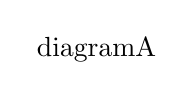
\begin{tikzpicture}
            \node at (0, 0) {{diagramA}};
        \end{tikzpicture}
    \end{center}
    \begin{tasks}(2)
        \task Option A
        \task Option B
        \task Option C\ans
        \task Option D
    \end{tasks}
